\documentclass[a4paper,10pt,twocolumn]{article}
%\documentclass[a4paper,10pt]{article}
\usepackage[pdftex]{graphicx}
\usepackage{float}
\usepackage{times}
\usepackage{color}
%\usepackage{fancyheadings}
%\restylefloat{figure}

%\oddsidemargin=0.1in
\topmargin=-0.8in
\textheight=9.8in
\textwidth=6.25in

\parskip 10pt
\parindent 0in

%\parskip 0pt
%\parindent 0.25in
\newif\ifdraft
%\drafttrue


\ifdraft
\newcommand{\fixme}[1]{ { \bf{ ***FIXME: #1 }} }
\newcommand{\note}[1]{ {\textcolor{red} { ***Jha: #1 }}}
\else
\newcommand{\jhanote}[1]{}
\newcommand{\note}[1]{}
\fi

\newcommand{\oldadvertservice}{\textit{OldAdvertService }}
\newcommand{\newadvertservice}{\textit{NewAdvertService }}

\begin{document}
\thispagestyle{plain}
\title{The SAGA Advert Service: Concepts, Implementations and Usage Modes}
\author{Hans-Christian~Wilhelm \footnotemark, Ole~Weidner\footnotemark \\ {\em \small{Center for Computation and Technology, Louisiana State University,}} \\ {\em {\small 216 Johnston Hall, Baton Rouge, LA 70803, USA}}
\\ {\footnotesize $^*$ hcwilhelm@cct.lsu.edu, $^\dag$ oweidner@cct.lsu.edu}}

\date{}

\maketitle


\begin{abstract}

\end{abstract}

\section{Introduction} 


\begin{figure*}[ht]
  \centering
  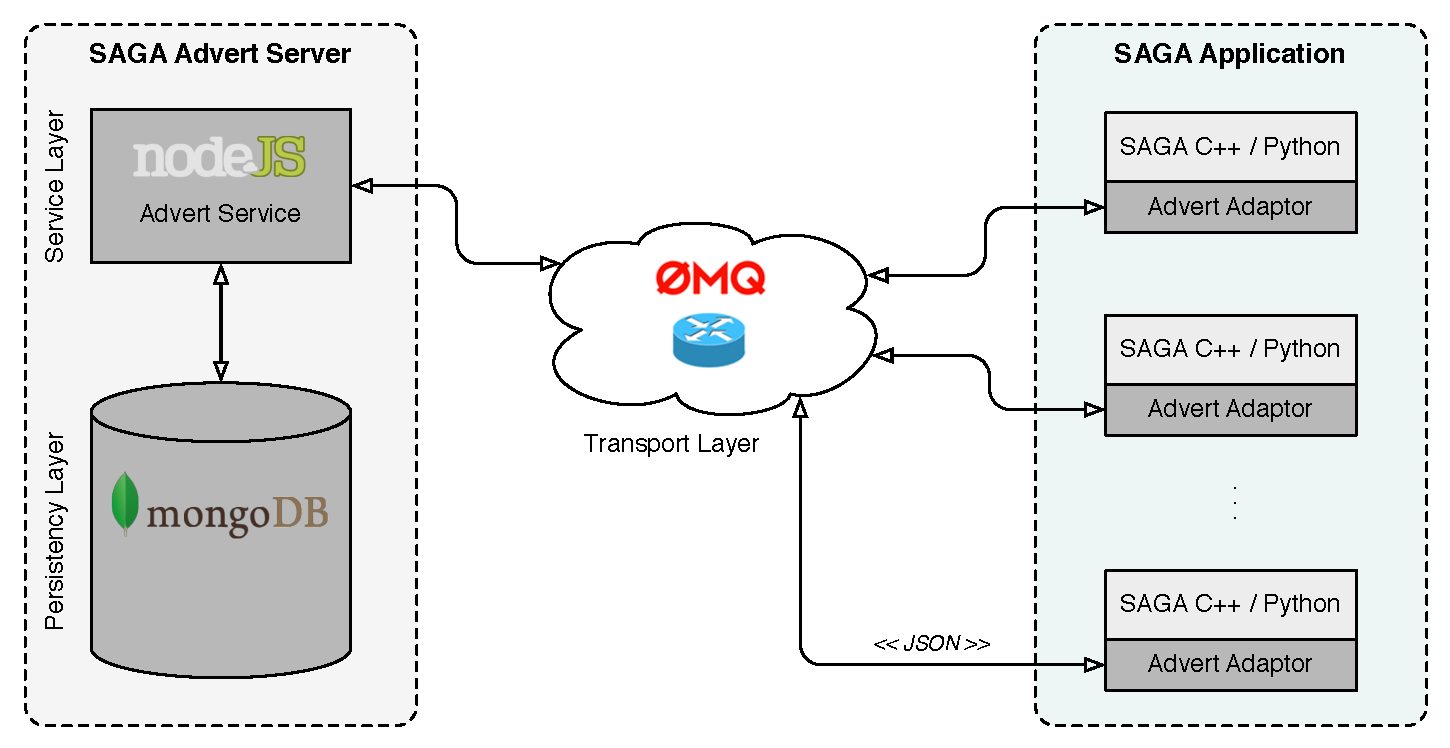
\includegraphics[width=3.0in]{figures/old_technology_overview} 
  \hspace{3 mm}
  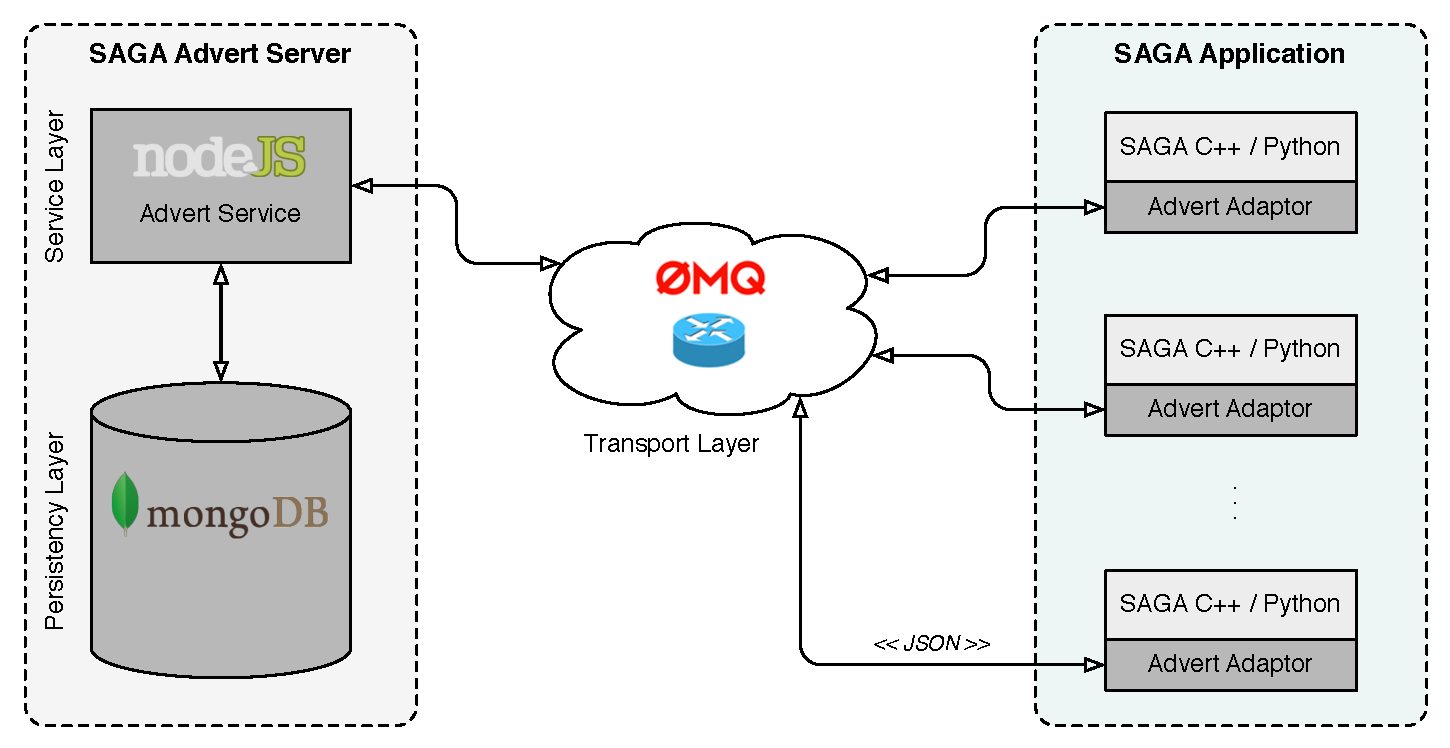
\includegraphics[width=3in]{figures/new_technology_overview}

  \caption[Architecture comparison of the \oldadvertservice and the \newadvertservice]%
  {Architecture comparison of the \oldadvertservice (left)and the \newadvertservice (right). The \oldadvertservice model implements direct communication between the advert adaptors and the persistence layer which is represented by a PostgreSQL database. The \newadvertservice uses \textit{node.js} as a distributed messaging service layer and  \O MQ (\textit{zero MQ}) on the transport layer. Persistency is established though a \textit{mongoDB} database below \textit{node.js}. }
\end{figure*}

\section{Specification (Andre)}
A.M: History, etc... 

\section{Implementations (Hans / Hartmut} 

- Hypertables, ... 

\subsection{Old}

\subsection{New}

\subsubsection{MPTT}

\subsubsection{Stored Procedures}

\subsection{Performance Evaluation}

\section{Usage Modes (Ole / Hartmut)}

(1) Communication (2) Synchronization (3) Data Exchange/Storage/Transfer

- what do we do with the advert service? 
- what are the application scenarios? 

- what is the difference between a advert service 

- serialization: job and endpoint serialization (see saga-shell)

\section{Application Examples (Shantenu)}

\thispagestyle{plain}
\end{document} 
